\section{Scaling actual-cause computation: an empirical comparison}\label{sec:ac_benchmark}

The correspondence in Theorems~\ref{th:ac-exp}--\ref{th:exp-ac} and
Proposition~\ref{prop:filter} is a statement about verdicts: under the stated
hypotheses, AC actual causes coincide with the support of $\sum_{\mathbf{T}}\Phi$.
This section reports an empirical companion to the correspondence. We ask whether
the necessity-only PCI kernel of Definition~\ref{def:ackernel}, instantiated with a
finite Monte Carlo estimator, recovers AC verdicts at problem sizes where exact
subset enumeration is no longer tractable. The full implementation, raw outputs and
plotting code are in the companion notebook
\texttt{docs/source/actual\_causality\_benchmark.ipynb}.

\medskip\noindent\textit{Generalised throwing problem.}
For a size parameter $n$ we replicate the canonical Sally/Billy structure $n$ times
in parallel. Binary suspects $A_1,\dots,A_n,B_1,\dots,B_n\in\{0,1\}$ feed
deterministic mediators
\(W^a_i = A_i,\quad W^b_i = B_i \land \lnot A_i\)
that capture overdetermination via preemption: $B_i$ contributes only if $A_i$ does
not. The outcome is the conjunction $C = \bigwedge_{i=1}^{n} (W^a_i \lor W^b_i)$, and
the model size grows as $4n+1$ variables. Ground-truth responsibility at site $i$ is
read off during the forward pass: $A_i$ is responsible if $W^a_i=1$, $B_i$ is
responsible if $W^b_i=1$. The structure scales the canonical example without softening it ---
overdetermination, undercutting, and witness-mediated symmetry-breaking are present
at every site --- while keeping a closed-form ground truth available for evaluation.

The variable partition takes the roots $\{A_i,B_i\}_i$ as suspects and the
deterministic mediators $\{W^a_i,W^b_i\}_i$ as witnesses, with no suspect a
deterministic function of the others. This partition satisfies the closure
condition required by Theorem~\ref{th:ac-exp} (see the Remark on deterministic
intermediates and joint support, which addresses precisely the scenario in which
both a root and its structural descendant are admitted as suspects). The
benchmark is therefore within the scope of the formal correspondence; in
particular, joint full support of the alternative-value distribution holds on the
admissible suspect set $\{A_i,B_i\}_i$ even though the model itself is
deterministic, because witnesses are not themselves part of the alternative-value
distribution.

\medskip\noindent\textit{Exact subset enumeration (AC reference).}
The exact procedure mechanises Definition~\ref{def:ac}: for each non-empty cause
subset $\mathbf{C}\subseteq\{A_i,B_i\}_i$ and each non-empty witness subset
$\mathbf{T}\subseteq\{W^a_i,W^b_i\}_i$, we intervene
$[\mathbf{C}\!\leftarrow\!\mathbf{1}-\mathbf{c}^\star,\mathbf{T}\!\leftarrow\!\mathbf{w}^\star]$,
record whether the outcome flips, and accept $\mathbf{C}$ as actual cause if some
witness $\mathbf{T}$ achieves a flip and no proper subset of $\mathbf{C}$ does.
The search space has $\bigl(2^{2n}-1\bigr)^2$ cause-witness pairs --- $9, 225, 3969,
65025$ for $n=1,2,3,4$ --- which already determines the ceiling reached by the exact
method.

\medskip\noindent\textit{Approximate PCI estimator.}
The PCI estimator instantiates the kernel of Definition~\ref{def:ackernel}
via Monte Carlo using the \texttt{ThinSearchSampler} of
Section~\ref{sec:causal_impact}. Algorithm~\ref{alg:pci_thin_search} is the
explicit procedure used to produce the curves in
Figures~\ref{fig:ac_runtime}--\ref{fig:ac_accuracy}.

\begin{algorithm}[ht]
\caption{Approximate PCI estimator on the scaled throwing problem.}
\label{alg:pci_thin_search}
\begin{algorithmic}[1]
\Require PSCM $M$; factual world
$(\mathbf{s}^\star,\mathbf{w}^\star,c^\star)$; cardinality bounds
$n_s, n_w$; sample budget $N$; witness flag
$\mathrm{wit}\in\{\text{on},\text{off}\}$
\Ensure per-site verdicts $v_i\in\{A_i,B_i\}$ for $i=1,\dots,n$
\If{$\mathrm{wit} = \text{off}$}
  \State $\mathbf{W} \gets \emptyset$ \Comment{no witness candidates}
\EndIf
\For{each $X\in\mathbf{S}$}
  \State $L[X] \gets [\,]$ \Comment{per-suspect score list}
\EndFor
\For{$j = 1,\dots,N$}
  \State draw $\mathbf{u}_j \sim P_{\mathbf{U}}$
  \State sample $k_s \sim \mathrm{Unif}\{1,\dots,n_s\}$,\quad
         $k_w \sim \mathrm{Unif}\{0,\dots,n_w\}$
  \State sample $\mathbf{C}_j \subseteq \mathbf{S}$ uniformly with
         $|\mathbf{C}_j| = k_s$
  \State sample $D_j \subseteq \mathbf{W}$ uniformly with $|D_j| = k_w$
         \Comment{witnesses dropped}
  \State $\mathbf{T}_j \gets \mathbf{W} \setminus D_j$
         \Comment{active witnesses}
  \State $\mathbf{c}'_j \gets \mathbf{1} - \mathbf{s}^\star\!\mid_{\mathbf{C}_j}$
         \Comment{bit-flip on $\{0,1\}$}
  \State $y^s_j \gets M.\mathrm{run}\bigl(\mathbf{u}_j,\,
         \mathrm{do}(\mathbf{C}_j = \mathbf{s}^\star\!\mid_{\mathbf{C}_j},\,
         \mathbf{T}_j = \mathbf{w}^\star\!\mid_{\mathbf{T}_j})\bigr)$
         \Comment{sufficiency}
  \State $y^n_j \gets M.\mathrm{run}\bigl(\mathbf{u}_j,\,
         \mathrm{do}(\mathbf{C}_j = \mathbf{c}'_j,\,
         \mathbf{T}_j = \mathbf{w}^\star\!\mid_{\mathbf{T}_j})\bigr)$
         \Comment{necessity, shared $\mathbf{u}_j$}
  \For{each $X \in \mathbf{C}_j$}
    \State append $|y^n_j - c^\star|$ to $L[X]$
  \EndFor
\EndFor
\For{each $X\in\mathbf{S}$}
  \State $\mathrm{score}[X] \gets \mathrm{nanmean}(L[X])$
\EndFor
\For{$i = 1,\dots,n$}
  \State $v_i \gets \arg\max\bigl(\mathrm{score}[A_i],\,\mathrm{score}[B_i]\bigr)$
\EndFor
\State \Return $(v_1, \dots, v_n)$
\end{algorithmic}
\end{algorithm}

The algorithm draws $N$ intervention configurations under shared noise.
The active suspect set $\mathbf{C}_j$ (line~6) is drawn at uniformly chosen
cardinality $k_s \in \{1,\dots,n_s\}$; the dropped witness set $D_j$
(line~7) is drawn the same way at $k_w \in \{0,\dots,n_w\}$, and the active
witnesses on line~8 are the complement $\mathbf{W}\setminus D_j$ --- so
$n_w$ bounds the number of witnesses \emph{dropped}, not the number kept,
and the active witness set has size $|\mathbf{W}|-n_w$ or larger. The
witness ablation flag $\mathrm{wit}=\text{off}$ is handled once on line~1
by emptying $\mathbf{W}$; this collapses the witness machinery on
lines~7--8 and 11--12 to no-ops, producing the dotted accuracy curves of
Figure~\ref{fig:ac_accuracy}.

Alternative values on line~9 are bit flips: on $\{0,1\}$ the
$\epsilon$-excised alternative-value distribution has a single support
point and $\epsilon$ plays no role; the explicit sampling form is preserved
so that the same routine runs on continuous benchmarks. The two
interventional worlds on lines~11--12 share the noise realisation
$\mathbf{u}_j$ drawn on line~4 --- the standard counterfactual coupling
--- which lets the per-suspect score on lines~14--16 be read off as the
nan-mean of $|y^n_j - c^\star|$ over the draws in which
$X\in\mathbf{C}_j$. The sufficiency outcome $y^s_j$ is computed but not
consumed: the AC verdict against which we benchmark has no sufficiency
clause, so we read only the necessity world. The joint estimator with
sufficiency active is exercised in Sections~\ref{sub:synthetic},
\ref{sec:DCE}, and~\ref{sec:sir_benchmark}, where AC has no comparable
verdict to benchmark against. At each site
$i = 1,\dots,n$, line~17 returns the suspect --- $A_i$ or $B_i$ --- with
the higher mean.

\medskip\noindent\textit{Benchmark protocol.}
For each problem size $n$ we sample up to ten distinct factive worlds (with
\(C=1\)), instantiate the model, run both methods to verdicts, and compare to the
analytic ground truth. Each method is granted a 60-minute global budget per run; if
the budget is exhausted mid-loop, the largest completed $n$ caps the curve. The
approximate estimator is exercised in five configurations that vary along three axes
identified in Section~\ref{sec:causal_impact}:
(i) initial sample budget $N_0\in\{250,500\}$, scaled linearly with $n$ by a factor
$\alpha\in\{0.5,1\}$ so that the total sample at size $n$ is $\alpha\cdot N_0\cdot n$;
(ii) presence of witness interventions ($\mathrm{wit}\in\{\text{on},\text{off}\}$),
ablating $\mathbf{T}\!\leftarrow\!\mathbf{w}^\star$ to test whether witness pinning is
load-bearing; (iii) cardinality bounds $n_s,n_w$, fixed at $4$ in the default runs
(answering ``does some witness set of size $\geq|\mathbf{W}|-4$ work?'') and grown
linearly as $4n$ in the dynamic-set-size configuration (recovering the unrestricted
subset search at the cost of higher variance). The cardinality bound is a tunable
approximation knob, not a hidden assumption: the dynamic-set-size run measures the
empirical cost of bounding $n_s,n_w$ at $4$ on this problem, and the gap between
the two configurations is what the ablation surfaces. The conceptual case for
constraining cardinality at all --- that uniform sampling over the full powerset
biases attributions toward large-coalition interventions and is analogous to
declining to enumerate all $n$-way regression interaction terms --- is given in
Section~\ref{sec:causal_impact}.

\medskip\noindent\textit{Results.}
Three observations summarise the experiment. First, runtime
(Figure~\ref{fig:ac_runtime}): the exact procedure times out at $4n+1=17$ variables
($n=4$) once the cause-witness search space crosses sixty-five thousand pairs, while
the approximate methods continue to roughly $73$--$145$ variables depending on
sample budget, with the frugal $\alpha{=}0.5$ run reaching the largest sizes.
Second, search-space size (Figure~\ref{fig:ac_search_space}, log scale): the exact
method visits the full powerset, while the approximate methods visit at most a few
hundred unique configurations per problem size --- the gap is several orders of
magnitude and widens with $n$. Third, accuracy (Figure~\ref{fig:ac_accuracy}): the
exact method is correct by construction up to its early demise; the witness-using
approximate methods stay above $0.85$ correct-attribution rate up to roughly $60$
variables and degrade gracefully beyond that, with the dynamic-set-size run
sustaining among the highest accuracies at moderate problem sizes. Witness-free
runs (dotted) underperform throughout, starting near $0.67$ already at $n=1$. The
ablation confirms a structural claim of Section~\ref{sec:causal_impact}: pinning
factual witness values is doing real work, not just regularising.

\begin{figure}[htbp]
\centering
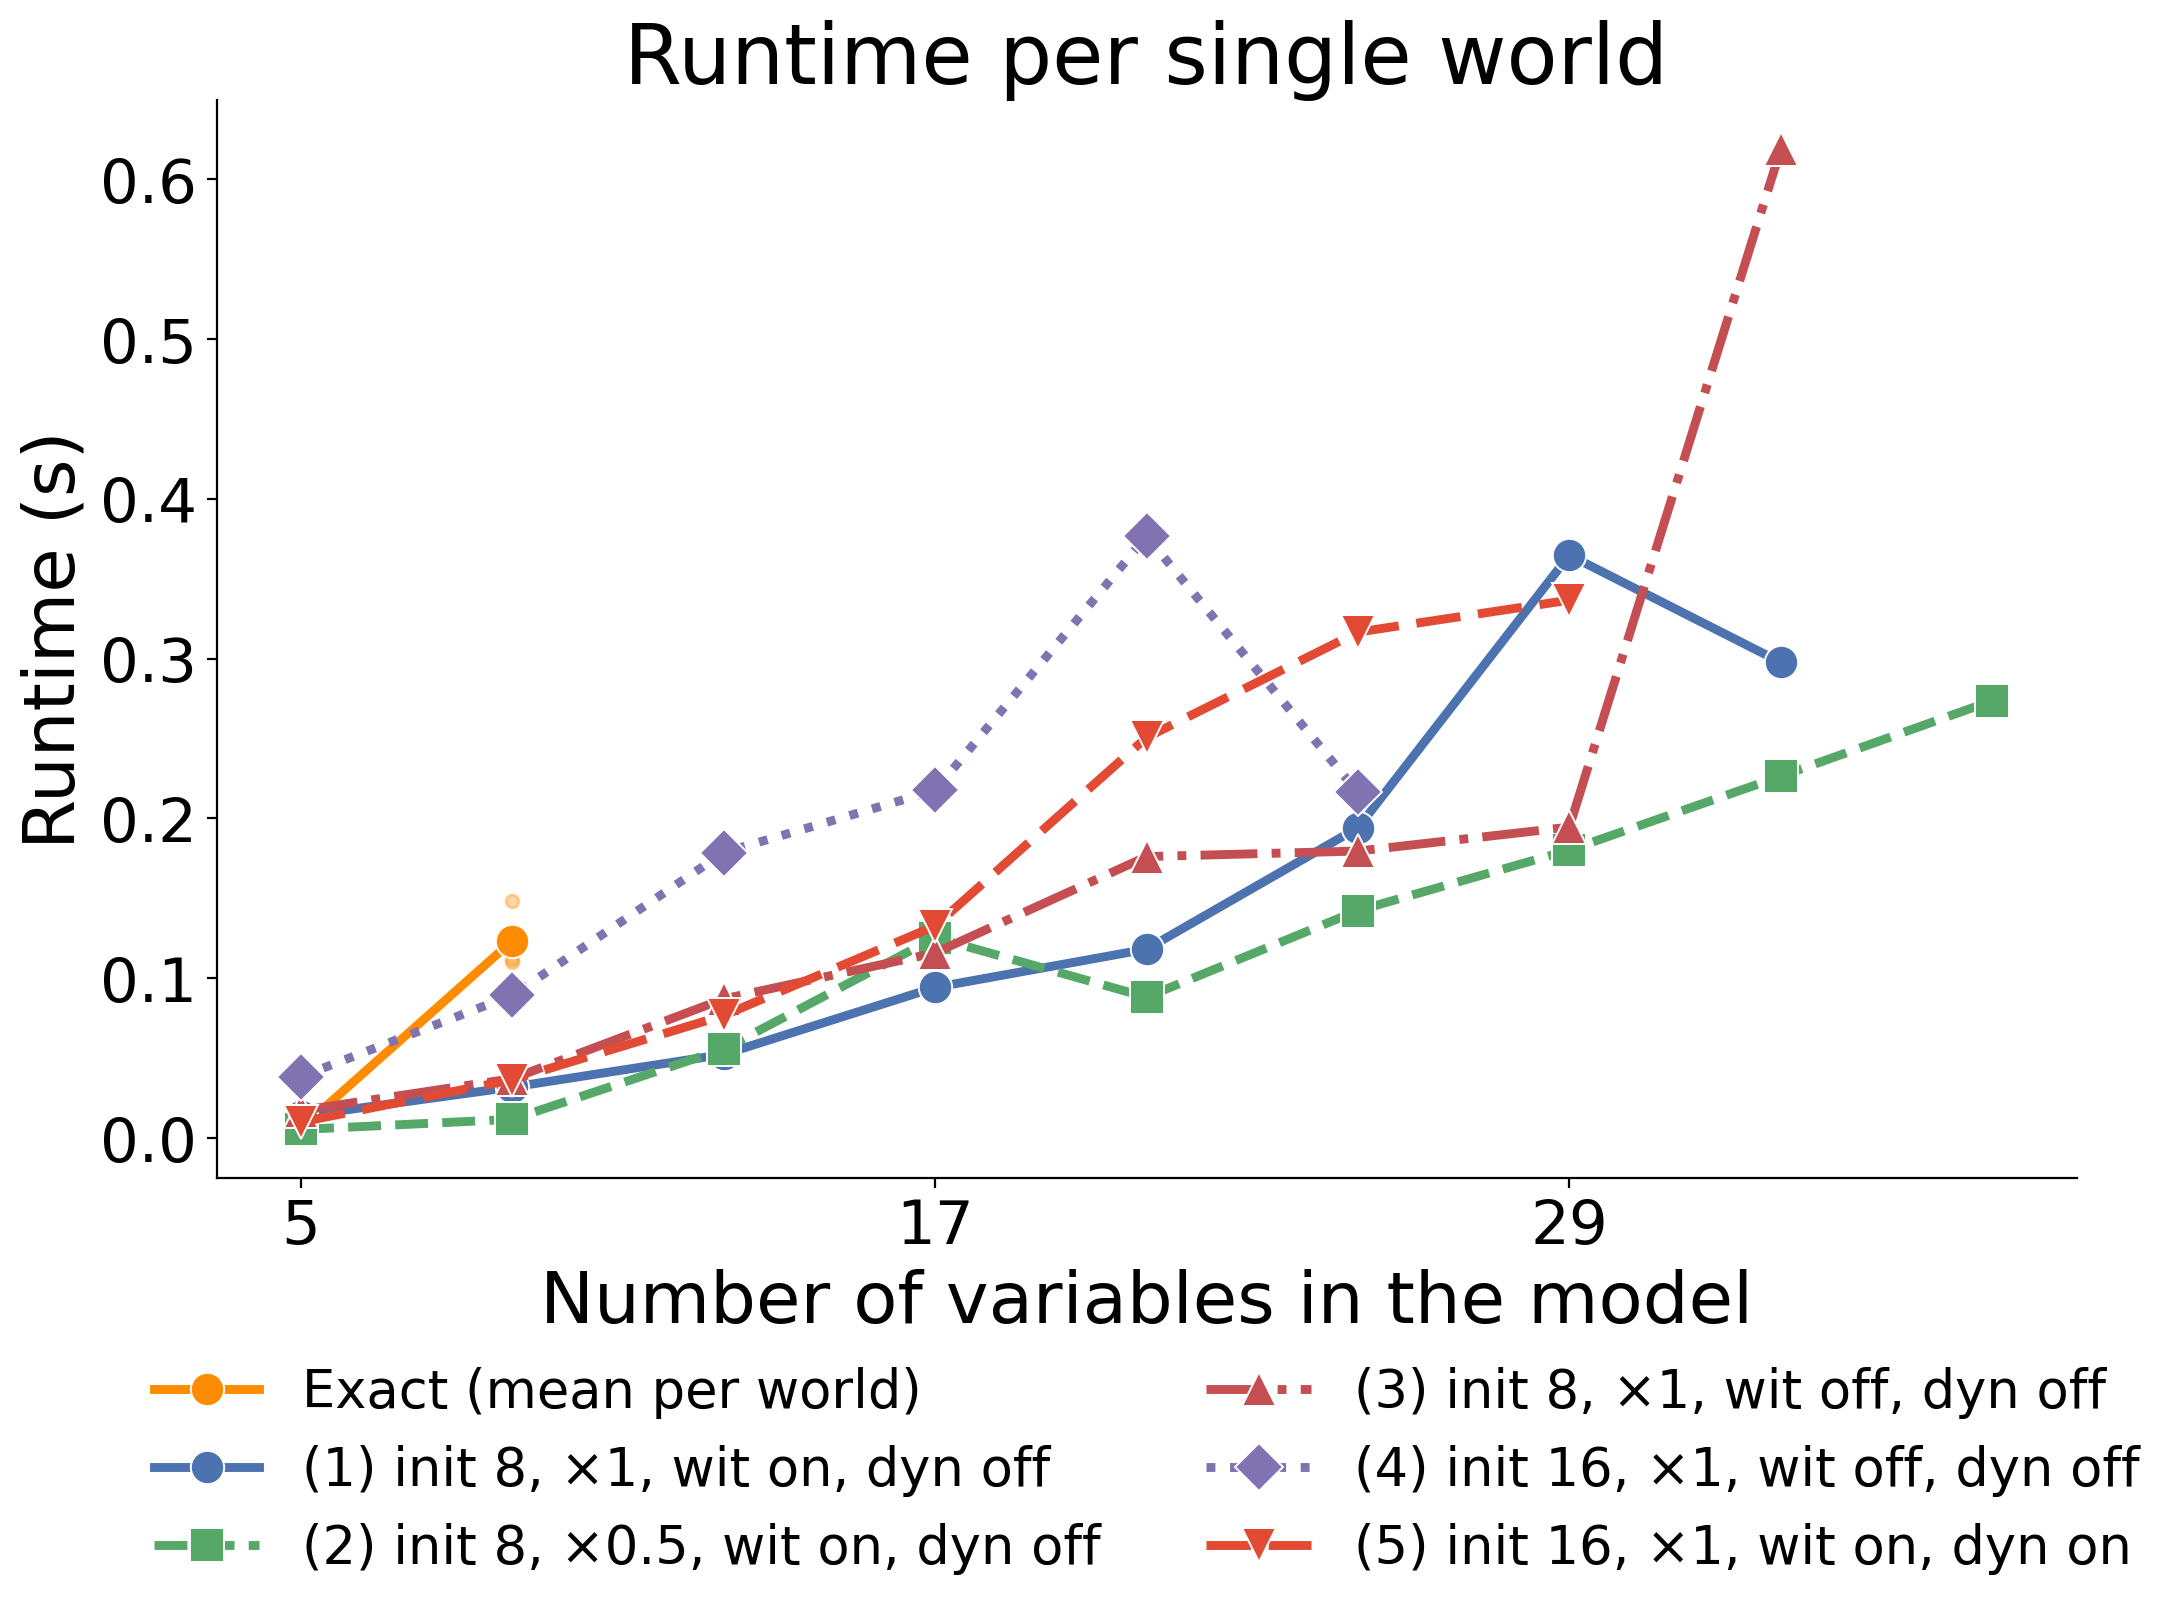
\includegraphics[width=0.92\linewidth]{docs/source/ac_benchmark/plot1_runtime.png}
\caption{Per-world runtime against problem size. The exact method (orange) times
out at 17 variables; approximate methods continue, with reach controlled by total
sample budget. Five approximate configurations vary initial sample size, the
linear-growth factor $\alpha$, the witness ablation, and dynamic cardinality
bounds; see Benchmark protocol.}
\label{fig:ac_runtime}
\end{figure}

\begin{figure}[htbp]
\centering
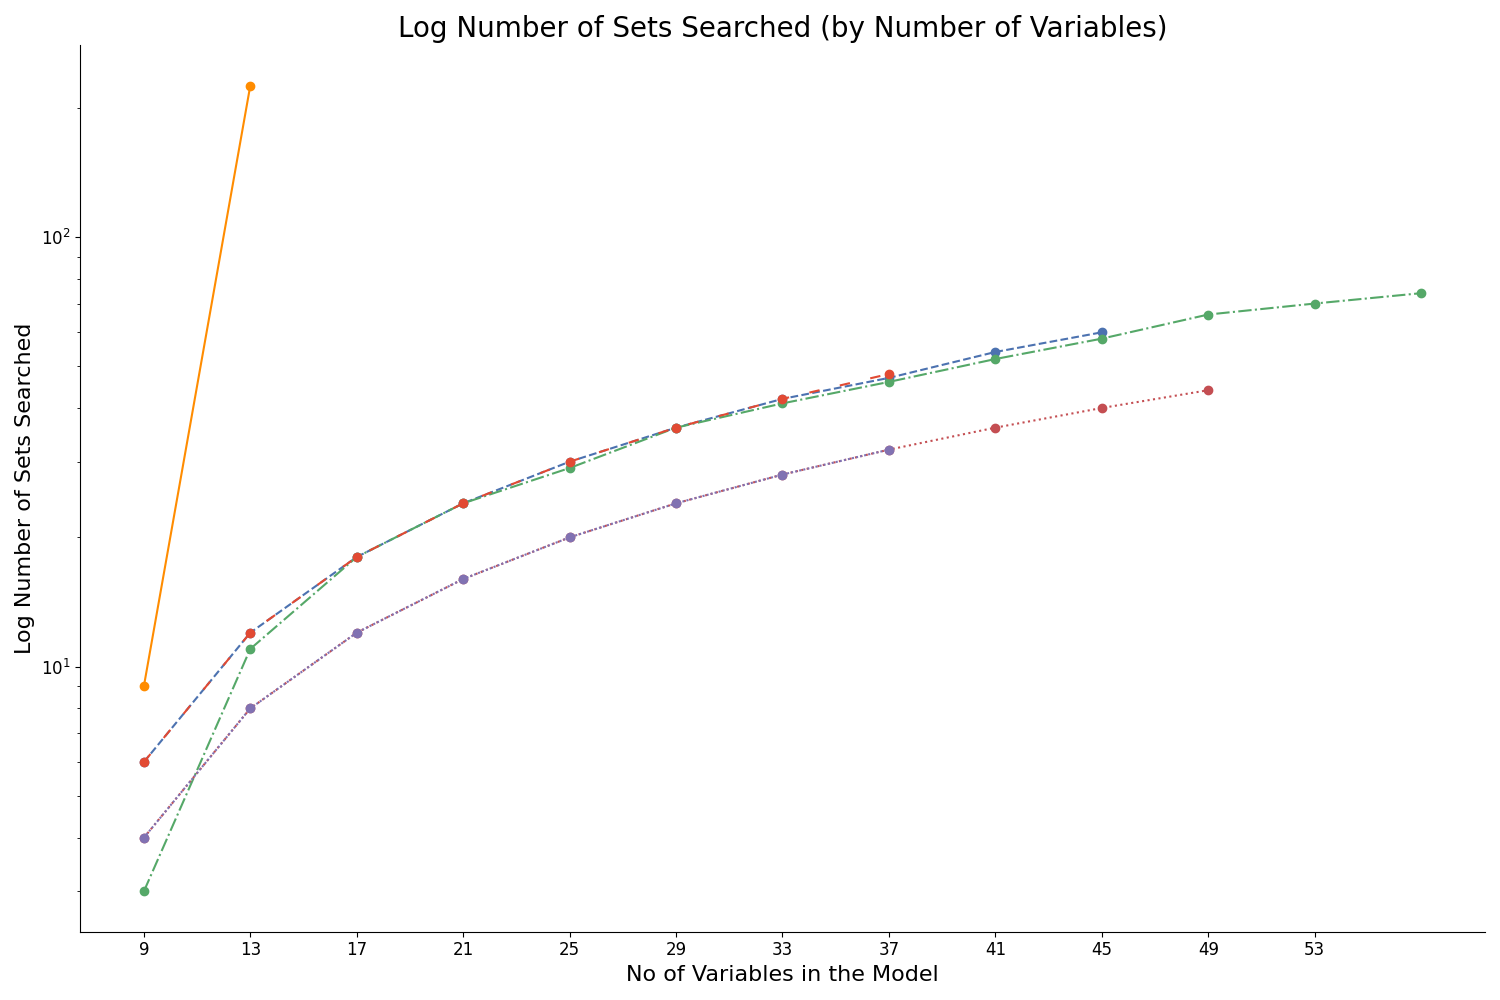
\includegraphics[width=0.92\linewidth]{docs/source/ac_benchmark/plot2_search_space.png}
\caption{Number of cause-witness configurations explored per problem size, log
scale. The exact method visits the full powerset; the approximate methods visit a
few hundred unique configurations per problem size regardless of $n$ --- a gap of
several orders of magnitude that grows with $n$.}
\label{fig:ac_search_space}
\end{figure}

\begin{figure}[htbp]
\centering
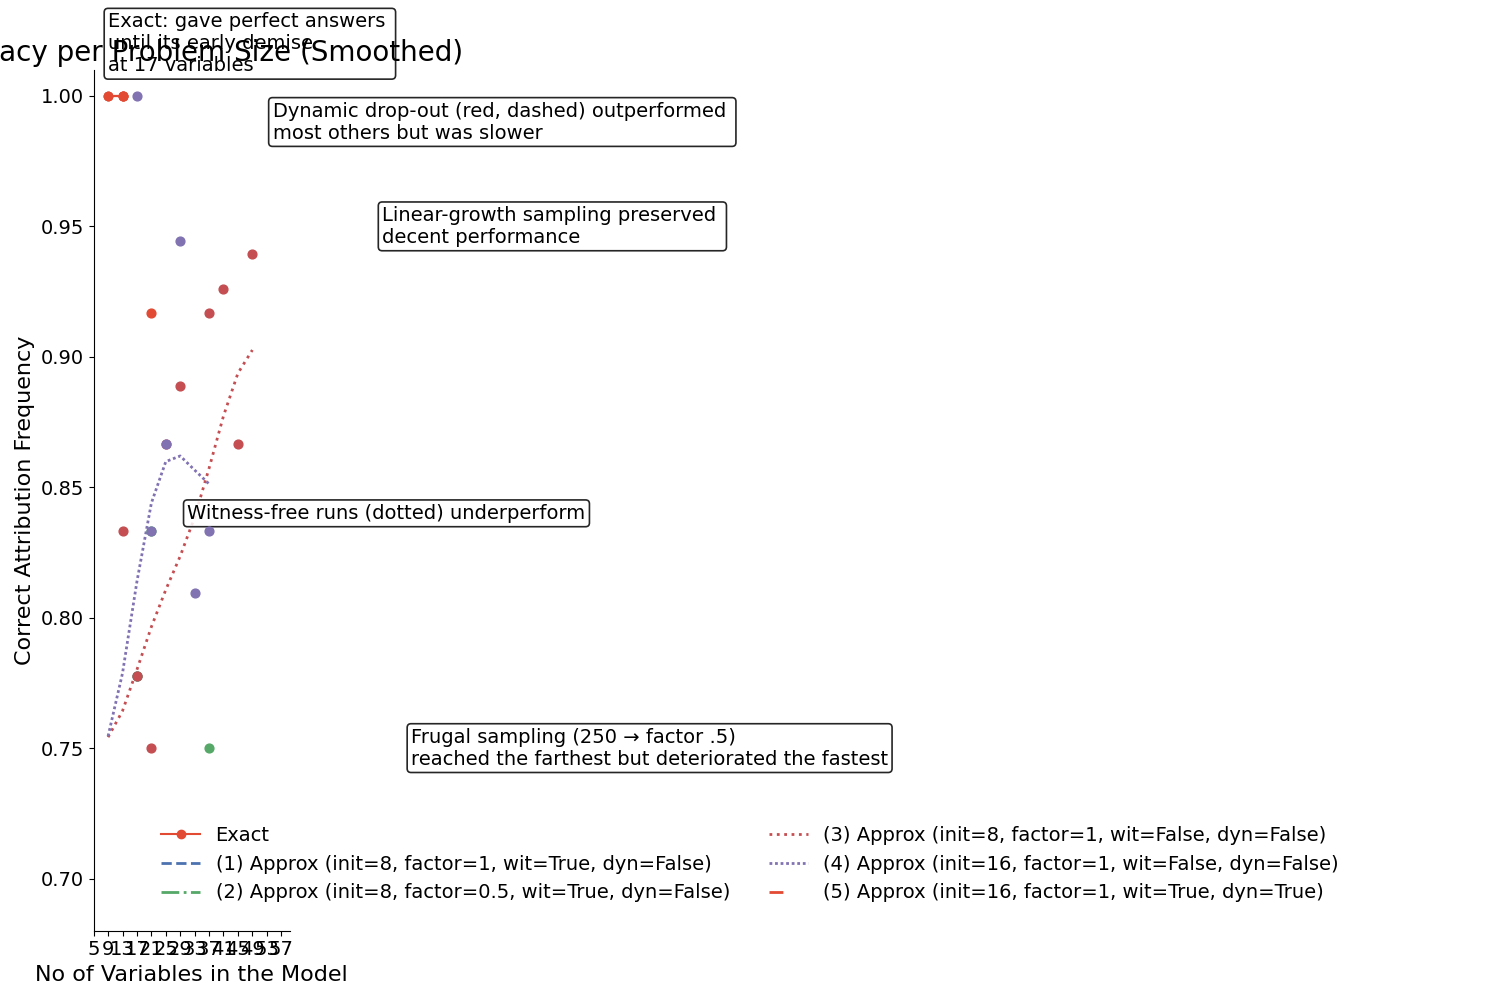
\includegraphics[width=0.92\linewidth]{docs/source/ac_benchmark/plot3_accuracy.png}
\caption{Correct-attribution rate against problem size, smoothed with a Gaussian
filter. The exact method is correct up to 17 variables. Witness-using approximate
runs stay above $0.85$ up to roughly 60 variables and degrade gracefully
thereafter; witness-free runs (dotted) underperform throughout, starting near
$0.67$. Dynamic-set-size sampling (dashed red) is among the highest at moderate
problem sizes.}
\label{fig:ac_accuracy}
\end{figure}

\medskip\noindent\textit{Scope of the conclusion.}
The benchmark establishes that the necessity-only PCI estimator tracks AC verdicts
on a faithful scaling of the canonical example with several orders of magnitude
fewer evaluated configurations. The problem itself, however, is structured:
responsibility attribution is independent across sites, exactly one of $A_i,B_i$ is responsible at
each site given $C{=}1$, supersets of any witness set witness the same attribution
(so a small witness-cardinality bound costs little), and all variables are binary.
These regularities account for some of the favourable scaling --- in particular,
the cardinality-bounded sampling losing little to dynamic-set-sizes sampling on
this problem. Two extensions are natural follow-ups. First, a comparison against
SHAP and causal SHAP on the same scaled-throwing problem is deferred to a
companion benchmark (cf.\ Section~\ref{sub:synthetic} for the corresponding
comparison on the continuous overdetermination example); the sufficiency component
of PCI is what distinguishes it from those baselines, and a clean head-to-head
requires the joint kernel rather than the necessity-only restriction used here.
Second, benchmarks that break each of the structural regularities above ---
particularly continuous-variable extensions where AC's mechanical enumeration is
no longer even well-defined --- would test the estimator outside its current
favourable regime. As a sanity check that the correspondence in
Theorems~\ref{th:ac-exp}--\ref{th:exp-ac} is empirically operational at scale, the
present comparison is sufficient.
